\documentclass[12pt, a4paper]{article}

\usepackage[a4paper, left=2.54cm, right=2.54cm, top=2.54cm, bottom=2.54cm]{geometry}
\usepackage[utf8]{inputenc}
\usepackage[T1]{fontenc}
\usepackage{mathptmx}
\usepackage[spanish]{babel}
\spanishdecimal{.}
\usepackage{setspace}
\doublespacing
\usepackage{indentfirst}
\usepackage{graphicx}
\usepackage{tikz}
\usetikzlibrary{positioning,arrows.meta,fit}

\setlength{\parindent}{1.27cm}

\newcommand{\fig}[2]{%
  \begin{minipage}[t]{0.485\textwidth}\vspace{0pt}\centering
  \includegraphics[width=\textwidth]{figuras/#1}\\[0.15em]
  {\small #2}
  \end{minipage}}

\begin{document}

\noindent
\begin{minipage}{0.82\textwidth}
    \textbf{David Sango Fuentes}\\
    Universidad Central del Ecuador -- Facultad de Ingeniería\\
    y Ciencias Aplicadas\\
    Carrera de Computación\\
    Materia: Fundamentos para Desarrollo de Videojuegos (Período 2026 - 2027)
\end{minipage}%
\begin{minipage}{0.18\textwidth}
    \raggedleft
    
\includegraphics[width=2cm]{logo_uce.png}
\end{minipage}

\vspace{0.35cm}
\begin{center}
    \textbf{\Large EVALUACIÓN SUMATIVA I}
\end{center}
\vspace{0.1cm}
\hrule
\vspace{0.6cm}

{\setstretch{1.3}
\begin{center}
{\large\textbf{Informe Técnico de Arquitectura}}\\[0.4em]
Proyecto integrador de medio semestre\\
\emph{La botella}: videojuego 2D en C++17 y SDL2\\[1.2em]
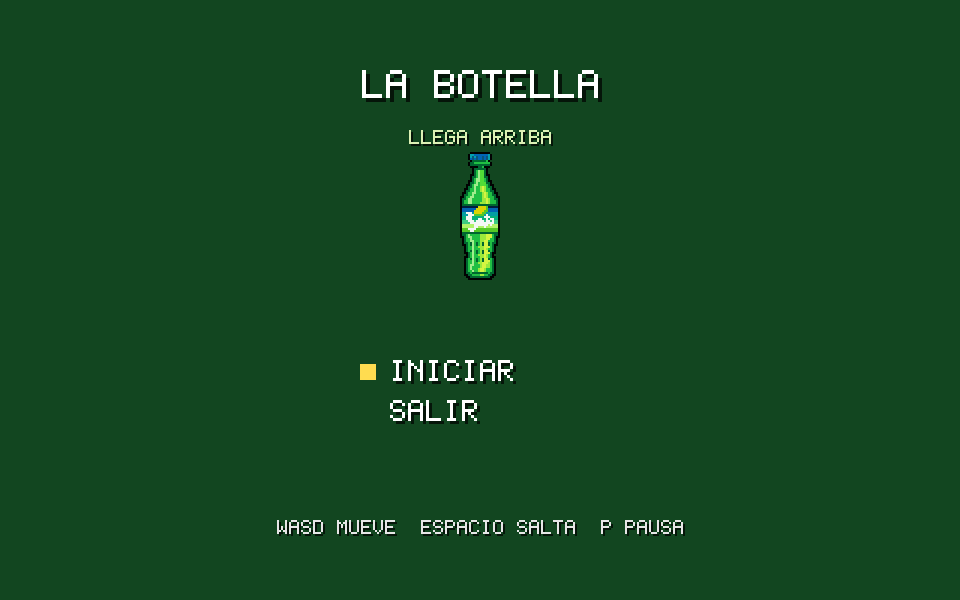
\includegraphics[width=0.62\textwidth]{figuras/fig_menu.png}\\[0.2em]
{\small Figura 1. Menú principal del juego.}\\[1.2em]
\begin{tabular}{rl}
Estudiante: & David Sango Fuentes\\
Código: & rama \texttt{sumativa-1-final}, carpeta \texttt{labs/s06\_sumativa\_i}\\
Fecha: & 27 de noviembre de 2026\\
\end{tabular}
\end{center}
}

\newpage

\section*{Qué se vio al jugar}

Al abrir el programa sale el menú \emph{La botella}. Con Enter empieza la partida. La botella aparece acostada en el pasto de abajo y la cámara la sigue mientras sube. Delante de ella hay una mira pequeña que marca dónde va a caer si salta. Arriba del todo está la meta.

Con A y D la botella gira en su sitio, sin moverse. Con W rueda hacia donde mira y con S retrocede; al soltar, el dibujo se queda en el cuadro en que estaba. La botella nunca se dibujó volteada en espejo. Mirando al norte, la consola marcó magnitud 1 y Dot Norte 0.9983; mirando en diagonal marcó 0.6413, con S $-0.6413$, y mirando al este casi 0. La magnitud siempre fue 1, así que la velocidad es la misma (250 px/s) en cualquier dirección.

Con Espacio la botella salta, crece y su sombra se queda en el suelo. Mientras más se sostiene W o S antes de saltar, más lejos va (de 1 a 4 celdas). Al caer sobre una caja, la caja desaparece y los puntos pasan de 0 a 10. Al entrar al agua la botella explota, las vidas bajan de 3 a 2 y vuelve al último pasto seguro. Al chocar con una caja la botella no explota: la caja la empuja a un lado y la botella se resbala por su borde. Con las tres vidas perdidas sale \emph{Fin del juego}. Con la tecla 1 el contador marcó entre 770 y 1060 cuadros por segundo, con la 2 unos 55 y con la 3 unos 28, y la botella siguió avanzando igual de rápido. En la pausa el mapa sigue a la vista pero nada se mueve.

{\setstretch{1}
\vspace{0.4em}
\noindent\fig{fig_juego.png}{Figura 2. Partida: HUD a la izquierda y mira delante de la botella.}\hfill
\fig{fig_salto.png}{Figura 3. Salto: la botella crece y la sombra queda abajo.}\\[0.8em]
\fig{fig_premio.png}{Figura 4. Después de caer, la caja ya no está y hay 10 puntos.}\hfill
\fig{fig_explota.png}{Figura 5. La botella explota al entrar al agua.}\\[0.8em]
\fig{fig_pausa.png}{Figura 6. Pausa con el mapa visible.}\hfill
\fig{fig_fin.png}{Figura 7. Fin del juego con 0 vidas.}\\[0.8em]
\fig{fig_hitbox.png}{Figura 8. Tecla H: cajas de choque (rojo sólido, azul agua, amarillo premio).}\hfill
\begin{minipage}[t]{0.485\textwidth}\vspace{0pt}\centering
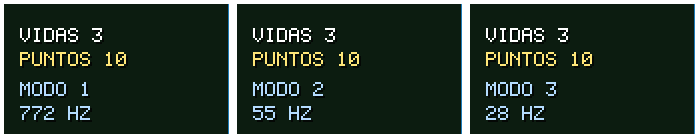
\includegraphics[width=\textwidth]{figuras/fig_fps.png}\\[0.15em]
{\small Figura 9. Teclas 1, 2 y 3: unos 770, 55 y 28 cuadros por segundo.}
\end{minipage}
\par}

\section*{Diagrama de clases}

El motor está en la carpeta \texttt{Engine/} y el juego en \texttt{Game/}. \texttt{Juego} une todo y \texttt{main.cpp} solo tiene el bucle.

{\setstretch{1}
\begin{center}
\begin{tikzpicture}[
    clase/.style={draw, align=center, inner sep=2pt, font=\scriptsize, text width=2.75cm, minimum height=9mm, fill=white},
    flecha/.style={-{Stealth[length=2mm]}, semithick},
    usa/.style={-{Stealth[length=2mm]}, dashed}
]
    \node[clase] (main) at (0,0) {\textbf{main.cpp}\\bucle de paso fijo};
    \node[clase] (juego) at (0,-1.5) {\textbf{Juego}\\une todo};
    \node[clase] (mapa) at (-6.15,-3.1) {\textbf{Mapa}\\mapa.txt y fondo};
    \node[clase] (obs) at (-3.08,-3.1) {\textbf{Obstaculos}\\árboles, agua, premios};
    \node[clase] (per) at (0,-3.1) {\textbf{Personaje}\\giro, avance, salto, muerte};
    \node[clase] (orden) at (3.08,-3.1) {\textbf{OrdenUI}\\pila de pantallas};
    \node[clase] (ui) at (6.15,-3.1) {\textbf{UI}\\menú, HUD, letreros};
    \node[clase] (burb) at (1.15,-4.7) {\textbf{Burbuja}\\mira, hija de la botella};
    \node[draw, dotted, fit=(main)(mapa)(ui)(burb), inner sep=5pt, label={[font=\footnotesize]above left:Game/}] {};

    \node[clase] (vec) at (-6.15,-6.7) {\textbf{Vector2D}\\posición y velocidad};
    \node[clase] (aabb) at (-3.08,-6.7) {\textbf{Aabb}\\choque y MTV};
    \node[clase] (mat) at (0,-6.7) {\textbf{Matrix3x3}\\traslación, giro, escala};
    \node[clase] (fuente) at (6.15,-6.7) {\textbf{Fuente}\\letras del HUD};
    \node[draw, dotted, fit=(vec)(fuente), inner sep=5pt, label={[font=\footnotesize]below left:Engine/}] {};

    \draw[flecha] (main) -- (juego);
    \draw[flecha] (juego) -- (mapa.north);
    \draw[flecha] (juego) -- (obs.north);
    \draw[flecha] (juego) -- (per);
    \draw[flecha] (juego) -- (orden.north);
    \draw[flecha] (juego) -- (ui.north);
    \draw[usa] (per.south -| burb.north) -- (burb.north);
    \draw[usa] (-0.75,-3.55) -- (-0.75,-6.25);
    \draw[usa] (-1.2,-3.55) -- (aabb.north east);
    \draw[usa] (burb.south) -- (burb.south |- mat.north);
    \draw[usa] (obs) -- (aabb);
    \draw[usa] (mapa) -- (vec);
    \draw[usa] (ui) -- (fuente);
\end{tikzpicture}\\[0.25em]
{\small Figura 10. Clases del motor y del juego. Flecha llena: tiene; flecha punteada: usa.}
\end{center}
\par}

\section*{Patrones aplicados}

\textbf{Bucle de paso fijo.} La lógica avanza siempre de 16.66 ms en 16.66 ms con un acumulador, y el dibujo mezcla la posición vieja y la nueva con alpha. Por eso la botella se movió igual de rápido con 1, 2 o 3, aunque los cuadros por segundo cambiaron mucho.

\textbf{Pila de estados.} \texttt{OrdenUI} guarda las pantallas en una pila: Menú, Juego, Pausa, Victoria y Derrota. La pausa se pone encima del juego, por eso el mapa se sigue viendo y la física se queda quieta.

\textbf{Padre e hijo con matrices.} La botella arma su matriz con traslación, rotación y escala. El giro usa $T(p)\cdot R\cdot T(-p)$ con el pivote en el centro, por eso gira en su sitio. La mira es hija de la botella: su lugar sale de $M_{\mathrm{hijo\_mundo}} = M_{\mathrm{padre}}\cdot M_{\mathrm{hijo\_local}}$, y al girar la botella la mira se va con ella.

\textbf{Física y choques.} El salto usa Euler semi-implícito con $g = 980$: primero cambia la velocidad y luego la altura. \texttt{isGrounded} impide saltar en el aire. Contra las cajas, \texttt{Aabb::mtv} empuja a la botella lo mínimo para sacarla, primero en X y luego en Y. Árboles y agua quitan una vida. El mapa se lee de \texttt{mapa.txt} (16 por 64 celdas) y cada celda pasa a píxeles con $\mathrm{unitScale} = 1/32$.

\textbf{Clases separadas.} Cada clase hace una sola cosa, así un cambio en el menú no toca la física. Las texturas se liberan al cerrar.

\section*{Manual de usuario y controles}

\textbf{Objetivo:} llegar a la parte de arriba del mapa sin perder las tres vidas. Cada caja recogida da 10 puntos. Para ganar hay que cruzar saltando de caja en caja: si el salto no cae sobre una caja, o cae en agua o en un árbol, la botella explota.

{\setstretch{1.15}
\begin{center}
\begin{tabular}{|l|l|}
\hline
\textbf{Tecla} & \textbf{Qué hace}\\ \hline
W / S o flechas, Enter & Menú: elegir opción y aceptar (Esc cierra)\\ \hline
A / D & Girar la botella en su sitio\\ \hline
W / S & Rodar hacia adelante / hacia atrás\\ \hline
Espacio & Saltar (sostener W o S antes = salto más largo)\\ \hline
P o Esc & Pausa (Enter o P sigue, Esc vuelve al menú)\\ \hline
1 / 2 / 3 & Cambiar la espera entre cuadros\\ \hline
H o F1 & Mostrar u ocultar las cajas de choque\\ \hline
Enter / Esc & En Victoria o Fin del juego: jugar otra vez / menú\\ \hline
\end{tabular}
\end{center}
\par}

\end{document}
